\documentclass[UTF8,titlepage]{article}
\usepackage{amsmath,amssymb,amsthm,amsfonts,amscd}
\usepackage{fontspec}
\setmainfont{Times New Roman}
\usepackage{graphicx}
\usepackage{titlesec}
\usepackage{makecell}
\usepackage{longtable}
\usepackage{xcolor}
\usepackage{tcolorbox}
\usepackage{soul}
\usepackage{adjustbox}
\usepackage{tcolorbox}
\usepackage{enumerate}
\usepackage{pdfpages}
\usepackage{float}
\usepackage{colortbl}
\usepackage{tabularx}
\usepackage{multirow}
\usepackage{pgfplots}
\numberwithin{figure}{section}
\usepackage[left=1.25in,right=1.25in,%
top=1in,bottom=1in]{geometry}
\usepackage{color}
\titleformat{\section}
  {\raggedright\LARGE\bfseries}{\thesection}{1em}{}
\title{Answer for Problem Set 1}
\author{Boyuan Zhao}
\begin{document}
\begin{center}
    {\LARGE \textbf{Answer of Problem Set 3}}\\  % 这就是你的标题
    {\normalsize Boyuan Zhao}\\  % 这就是你的名字
    {\small \today}  % 这是日期
\end{center}
\section{Problem 1. Expenditure Minimization.}
\begin{enumerate}
    \item The partial derivative of the utility function with respect to $x_1$ is given by:
    \begin{align*}
        \frac{\partial u}{\partial x_1} &= \frac{1}{2} (x_1 x_2 x_3)^{-\frac{1}{2}} \cdot x_2 x_3 = \frac{x_2 x_3}{2 \sqrt{x_1 x_2 x_3}} \\
        \frac{\partial^2 u}{\partial x_1^2} &= -\frac{1}{4} (x_1 x_2 x_3)^{-\frac{3}{2}} \cdot x_2^2 x_3^2 = -\frac{x_2^2 x_3^2}{4 (x_1 x_2 x_3)^{3/2}}
        \end{align*}
        
    Therefore, the utility function is increasing in $x_1$ (since the first derivative is positive), and is concave in $x_1$ (since the second derivative is negative).
    
    \item The expenditure minimization problem is given by:
    \begin{equation*}
        \min_{x} p \cdot \textbf{x} \quad \text{s.t.} \quad u(\textbf{x}) = \bar{u}
        \end{equation*}
        
    \item The Lagrangian function for this problem is:
    \begin{equation*}
        \mathcal{L}(\textbf{x}, \lambda) = p \cdot x + \lambda(\bar{u} - u(\textbf{x}))
        \end{equation*}
    
    \item The first order conditions are given by:
    \begin{align*}
        \frac{\partial \mathcal{L}}{\partial x_i} &= p_i - \lambda \frac{\partial u}{\partial x_i} = 0 \\
        \frac{\partial \mathcal{L}}{\partial \lambda} &= \bar{u} - u(x) = 0
        \end{align*}
    \item compute the partial derivatives of the utility function:
    \begin{align*}
        p_1 - \lambda \frac{x_2 x_3}{2\sqrt{x_1 x_2 x_3}} &= 0 \\
        p_2 - \lambda \frac{x_1 x_3}{2\sqrt{x_1 x_2 x_3}} &= 0 \\
        p_3 - \lambda \frac{x_1 x_2}{2\sqrt{x_1 x_2 x_3}} &= 0
        \end{align*}
        
        Next, set the partial derivatives equal to each other and solve for the relationship between $x_1, x_2, x_3$:
        \begin{align*}
            \frac{p_1}{p_2} &= \frac{x_2 x_3}{x_1 x_3} \Rightarrow x_1 = \frac{p_2}{p_1} x_2 \\
            \frac{p_1}{p_3} &= \frac{x_2 x_3}{x_1 x_2} \Rightarrow x_3 = \frac{p_2}{p_3} x_2 \\
            \end{align*}
        Substitute the relationship between $x_1, x_2, x_3$ into the utility function:
        \begin{align*}
            \bar{u} &= \sqrt{x_1 x_2 x_3} \\
            &= \sqrt{\left(\frac{p_2}{p_1} x_2\right) \cdot x_2 \cdot \left(\frac{p_2}{p_3} x_2\right)} \\
            &= \sqrt{\left(\frac{p_2^2}{p_1 p_3}\right) x_2^3} \\
            &= \frac{p_2}{\sqrt{p_1 p_3}} x_2^{3/2} \\
            \end{align*}
            Finally, solve for $x_2$ to get $h_2$, and use $h_2$ to find $h_1$ and $h_3$:
            \begin{align*}
                h_1 &= \left(\frac{\bar{u} \sqrt{p_2 p_3}}{p_1}\right)^{2/3} \\
                h_2 &= \left(\frac{\bar{u} \sqrt{p_1 p_3}}{p_2}\right)^{2/3} \\
                h_3 &= \left(\frac{\bar{u} \sqrt{p_1 p_2}}{p_3}\right)^{2/3} \\
                \end{align*}
                
    \item Compute the derivatives and determine whether goods are substitutes or complements:
    \begin{align*}
        \frac{\partial h_1(p; \bar{u})}{\partial p_2} &= \frac{1}{3} \left(\frac{\bar{u} \sqrt{p_3}}{p_1 p_2}\right)^{2/3} \geq 0 \\
        \frac{\partial h_1(p; \bar{u})}{\partial p_3} &= \frac{1}{3} \left(\frac{\bar{u} \sqrt{p_2}}{p_1 p_3}\right)^{2/3} \geq 0  \\
        \end{align*}
        Here we see that $h_1$ increases with $p_2$ and $p_3$, so $x_1$ and $x_2$ are net substitutes while $x_1$ and $x_3$ are net substitutes.
    \item The expenditure function is given by the sum of prices times the quantities:
    \begin{align*}
        e(\textbf{p}; \bar{u}) &= p_1 h_1(\textbf{p}; \bar{u}) + p_2 h_2(\textbf{p}; \bar{u}) + p_3 h_3(\textbf{p}; \bar{u})
        \end{align*}
    \item First, substitute the Hicksian demand functions into the expenditure function:
    \begin{align*}
        e(p; \bar{u}) &= p_1 h_1(p; \bar{u}) + p_2 h_2(p; \bar{u}) + p_3 h_3(p; \bar{u}) \\
        &= 3 \left(\bar{u} \sqrt{p_1 p_2 p_3}\right)^{2/3}
        \end{align*}
        Then substitute $\bar{u}$ with $v(\textbf{p}; M)$ and set the expenditure equal to $M$:
        \begin{align*}
            M &= 3 \left(v(\textbf{p}; M) \sqrt{p_1 p_2 p_3}\right)^{2/3}
            \end{align*}
            
        Rearranging to isolate $v(\textbf{p}; M)$ and considering that the terms under each cube root in the equation are the same, we get:
        \begin{align*}
            v(\textbf{p}; M) &= \frac{M \sqrt{3M}}{9\sqrt{p_1 p_2 p_3}}
            \end{align*}
        \item Derive the Marshallian demand functions:
        \begin{align*}
            x_1^*(\textbf{p}; M) &= - \frac{\frac{\partial v(\textbf{p}; M)}{\partial p_1}}{\frac{\partial v(\textbf{p}; M)}{\partial M}} = \frac{M}{3p_1} \\
            x_2^*(\textbf{p}; M) &= - \frac{\frac{\partial v(\textbf{p}; M)}{\partial p_2}}{\frac{\partial v(\textbf{p}; M)}{\partial M}} = \frac{M}{3p_2} \\
            x_3^*(\textbf{p}; M) &= - \frac{\frac{\partial v(\textbf{p}; M)}{\partial p_3}}{\frac{\partial v(\textbf{p}; M)}{\partial M}} = \frac{M}{3p_3} \\
        \end{align*}  
        \item Compute these derivatives:
        \begin{align*}
            \frac{\partial x_1^*(\textbf{p}; M)}{\partial M} &= \frac{1}{3p_1} > 0\\
            \frac{\partial x_2^*(\textbf{p}; M)}{\partial M} &= \frac{1}{3p_2} > 0\\
            \frac{\partial x_3^*(\textbf{p}; M)}{\partial M} &= \frac{1}{3p_3} > 0\\
        \end{align*}
        As $\frac{\partial x_i^*}{\partial M}$ are all positive, goods $x_1, x_2, x_3$ are normal goods.
        \item In general, economic theory suggests that the quantity demanded for a good decreases as its price increases, all other things being equal. This is known as the law of demand. This implies that the derivatives $\partial x_i(p;M) / \partial p_i$ should be negative.
\end{enumerate}
\clearpage
\section{Problem 2. Expenditure minimization: tricky cases.}
\begin{enumerate}
    \item (a) In this case, the utility of the consumer is determined by the smaller of the two quantities $x_1$ and $x_2$. Therefore, for the consumer to achieve a certain level of utility u, it is necessary that $x_1$ = $x_2$ = $\bar{u}$ Therefore, $h_1$ = $h_2$ = $\bar{u}$

(b) In this situation, $h_1$ and $h_2$ are not dependent on $p_1$ and $p_2$. They only depend on the level of utility u that the consumer wants to achieve. Hence, the partial derivatives of $h_1$ and $h_2$ with respect to $p_1$ and $p_2$ are zero. The substitution effect of a change in price is zero because the consumer will always consume equal amounts of both goods.

The graph is shown below:
\begin{figure}[H]
\centering
 \resizebox{0.75\textwidth}{!}{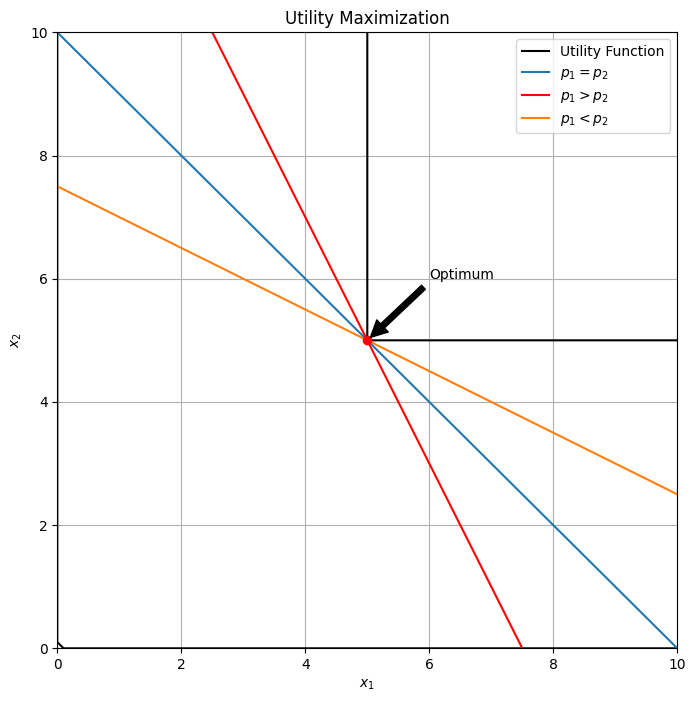
\includegraphics{/workspaces/TexFile/Microeconomic/graph/3.2.1.png}}
 \caption{The graph of $h_1$ and $h_2$}
 \label{}
\end{figure}
    \item In this case, the utility of the consumer is determined by the sum of the squares of $x_1$ and $x_2$. The consumer will try to distribute his expenditure in such a way that he maximizes his utility. Therefore, the consumer will consume more of the good which has lower price per unit. This is because, for the same amount of money, he can consume more of the good with lower price, and hence increase his utility. Therefore, the Hicksian compensated demand functions $h_1$ and $h_2$ will depend on the relative prices $p_1$ and $p_2$.
The graph is shown below:
\begin{figure}[H]
\centering
 \resizebox{0.75\textwidth}{!}{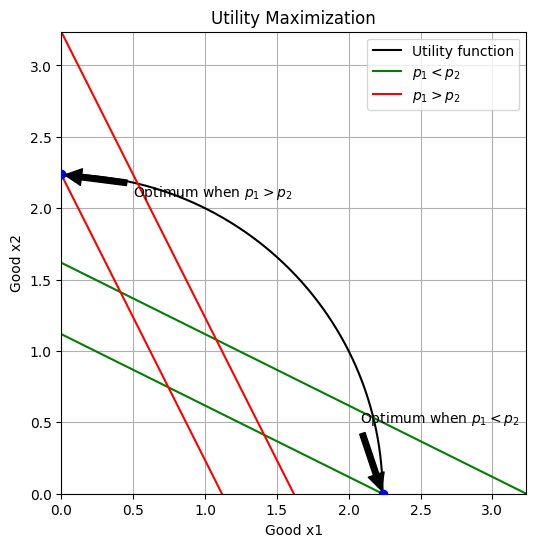
\includegraphics{/workspaces/TexFile/Microeconomic/graph/3.2.2.png}}
 \caption{The graph of $h_1$ and $h_2$}
 \label{}
\end{figure}
\end{enumerate}
\end{document}